
% =======================================================================================================
\documentclass{article}
% =======================================================================================================

\usepackage{my_personal_style} %


\setlength{\textheight}{9.0in}      %
\setlength{\textwidth}{7.0in}       %
\setlength{\oddsidemargin}{-0.25in} %
\setlength{\topmargin}{0.25in}      %
\setlength{\headsep}{-0.5in}        %
\setlength{\parindent}{0.25in}      %



\title{Title}
\author{Name}
\date{April 23, 2008}

% =======================================================================================================
\begin{document}
% =======================================================================================================

\maketitle %

\noindent \rule{7.0in}{.02in} %
\noindent \rule[.2in]{7.0in}{.03in} %

\tableofcontents %

\bigskip

\noindent \rule{7.0in}{.03in} %
\noindent \rule[.2in]{7.0in}{.02in} %

\newpage


% -------------------------------------------------------------------------------------------------------
\section{Overview}\label{overview}
% -------------------------------------------------------------------------------------------------------

The purpose of this document is to give a quick overview of the
basics needed to create reasonable LaTeX documents. It is not the
goal of this document to approach completeness or even to give a
rigorous treatment of LaTeX, but rather to provide a series of
examples that will quickly allow someone to create reasonable
looking LaTeX documents. LaTeX is more of a ``learn as you go''
kind of system. That being said, you should know that LaTeX is
extremely powerful and it should be possible to do almost anything
you can think of. Furthermore, in most cases, you can find a
package that will suit your needs in this regard.


I recommend that you use WinEdt to edit documents and that you use
MiKTeX to produce documents (e.g., in pdf or ps form).

(Note that I like to add comment-level separators to LaTeX
documents. I do this because it helps me visually parse raw LaTeX
documents.)

% -------------------------------------------------------------------------------------------------------
\section{Fonts}
% -------------------------------------------------------------------------------------------------------

Fonts can be altered in a variety of ways. Some examples include:
Code is oftentimes denoted using \texttt{this} font. Emphasis is
also \emph{very} useful, but not as \textbf{dramatic} as bolded
font. Of course, \underline{underlining} is also possible.

One can even change the {\Large size} of fonts. I have found that
{\tiny tiny} fonts can be hard to read. Fonts that are simply
{\small small} are a bit better. While {\Huge huge} fonts are
``out of control''\footnote{Notice how double open/close quotes
are denoted in LaTeX}. Overall, changing the size of a font should
be avoided.

And finally, these things can be \textbf{\emph{combined}}.

% -------------------------------------------------------------------------------------------------------
\section{Basic Layout}
% -------------------------------------------------------------------------------------------------------

Some basic layout mechanisms include: \emph{boxes},
\emph{minipages}, \emph{centering}, and a variety of spacing
commands.

% -------------------------------------------------------------------------------------------------------
\subsection{Box, Minipage, and Center}
% -------------------------------------------------------------------------------------------------------

The \fbox{command} is quite useful for enclosing elements within a
box. This can be applied to tables, but does not work very well
for paragraphs.

\begin{center}
Text can also be centered.
\end{center}

The minipage is a very useful mechanism for grouping portions of a
LaTeX document. For example, in a table a minipage can be used to
put a paragraph text within a cell. See Section
\ref{section-tables} for an example of this.

\bigskip

\begin{center}
\fbox{
\begin{minipage}{3.5in}
This text is part of a minipage whose width is 3.5 inches. This
minipage can be placed in a variety of locations, including in the
cell of a table. Furthermore, the minipage can be enclosed in an
fbox.
\end{minipage}
}
\end{center}


% -------------------------------------------------------------------------------------------------------
\subsection{Spacing}
% -------------------------------------------------------------------------------------------------------

There are a variety of commands that can be used to control both
horizontal as well as vertical spacing. The commands I use most
are: bigskip, medskip, smallskip, vspace, hspace


The command \hspace{5mm} will insert 5 mm of horizontal space. The
command

\vspace{25mm}

will insert 25 mm of vertical space. The skip commands can be used
to insert small amounts of vertical space.

\noindent The bigskip command

\bigskip

\noindent inserts this much space, while the medskip command

\medskip

\noindent inserts this much space.



% -------------------------------------------------------------------------------------------------------
\section{Basic Structures}
% -------------------------------------------------------------------------------------------------------

There are a few basic structures that are useful for creating
documents: lists, tables, and figures.


% -------------------------------------------------------------------------------------------------------
\subsection{Lists}
% -------------------------------------------------------------------------------------------------------

Lists come in two basic flavors: enumerate and itemize.


\begin{itemize}
\item The first item. %
\item The second item. %
\end{itemize}

\bigskip

\begin{enumerate}
\item The first enumerated item. %
\item The second enumerated item. %
\end{enumerate}


% -------------------------------------------------------------------------------------------------------
\subsection{Tables}\label{section-tables}
% -------------------------------------------------------------------------------------------------------

Tables can have one or more columns and rows/columns can be
separated by lines. A newline symbol can be used to terminate the
row of a table.

\bigskip

\begin{center}
\fbox{
\begin{tabular}{lll} %
\multicolumn{3}{c}{Title of My Table} \\ \hline %
Column 1 & Column 2 & Column 3 \\ \hline %
x        & y        & z        \\ %
\end{tabular}
} \
\end{center}

\bigskip

Cell contents can be justified either left (l), right (r), or
center (c). Cell contents can also be separated horizontally by
including the vertical bar $|$ in the table template.

\begin{center}
\begin{tabular}{|c|r|}
\hline %
gas            & \$ 45.00  \\ %
airfare        & \$1645.00 \\ \hline %
\textbf{Total} & \$1690.00 \\ \hline %
\end{tabular}
\end{center}

% -------------------------------------------------------------------------------------------------------
\section{Math}
% -------------------------------------------------------------------------------------------------------

One of the big strengths of LaTeX is its math display
capabilities. Here I just touch on the absolute basics. First, a
math environment can be created by enclosing text with the dollar
sign. For example, $x + y$ is a math environment. Basic
capabilities include subscripts $x_{sub}$ and superscripts
$x^{super}$. One can also do sub-sub scripts $x_{y_{sub}}$ though
care should be taken. Similarly, super-super scripts can also be
created.

Note that text in a math environment is slightly different from
emphasized text: $different$ versus \emph{different}. Also note
that in a math environment spaces are largely ignored $hello
world$. However, you can force a space with a backslash as
follows: $hello\ world$.


% -------------------------------------------------------------------------------------------------------
\section{Graphics}
% -------------------------------------------------------------------------------------------------------

Graphics can be included in a variety of ways. The way I use most
often is through the includegraphics command.

\begin{center}
\fbox{
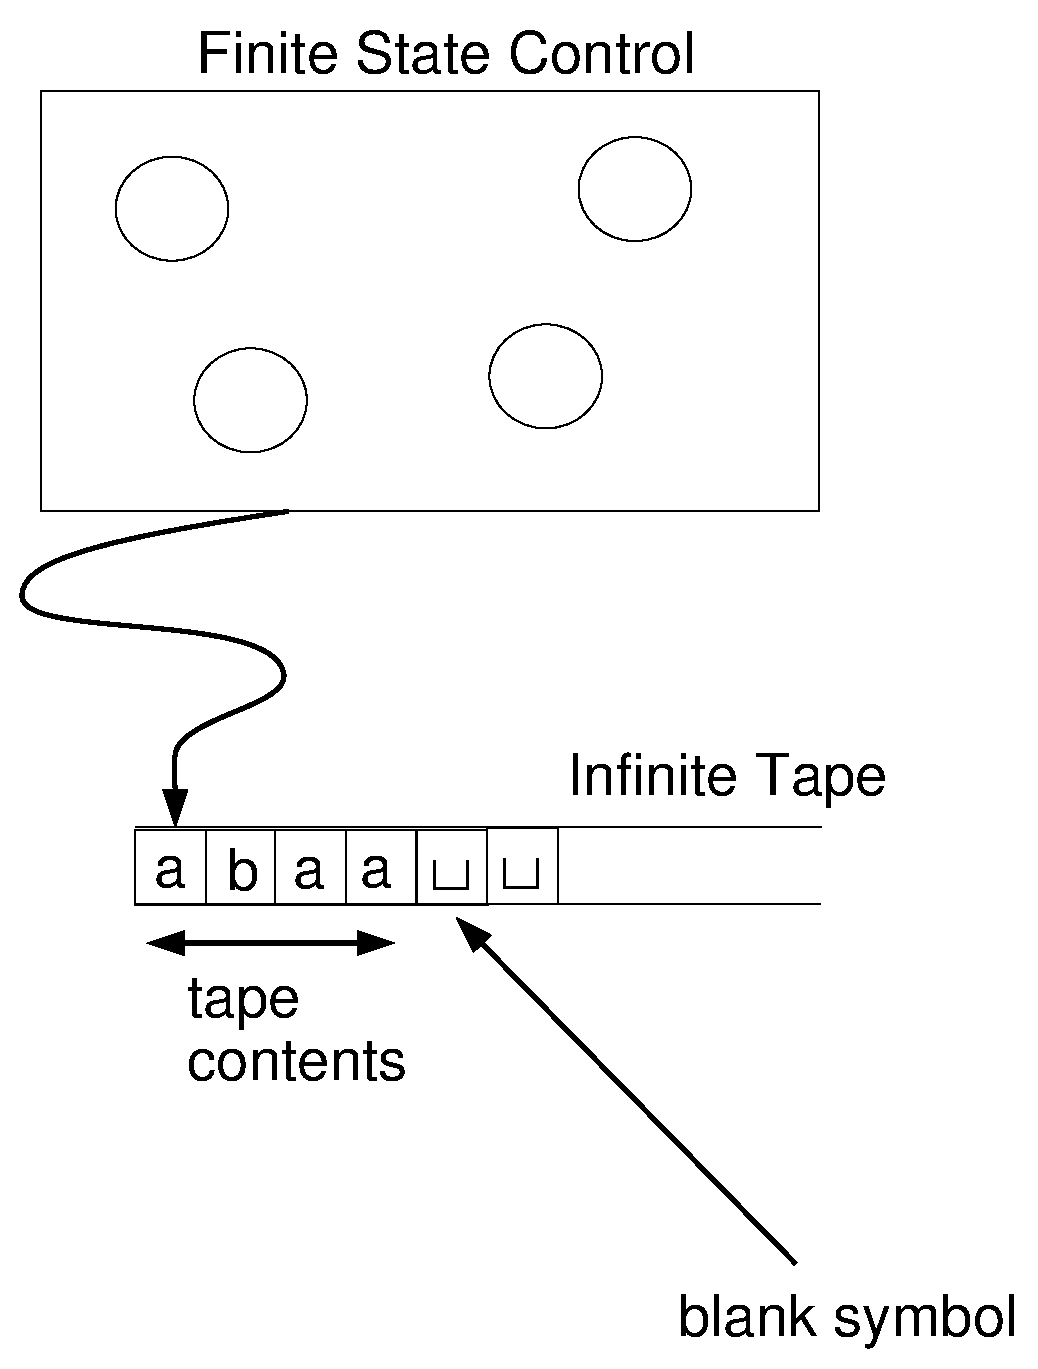
\includegraphics[scale=0.4]{mayura_draw_figure} %
}
\end{center}

Typically, I produce figures in pdf format using mayura draw.
However, note that other formats are also possible.

% -------------------------------------------------------------------------------------------------------
\section{Cross-referencing and Citations}
% -------------------------------------------------------------------------------------------------------

Labels can be assigned to a variety of constructs. For example,
figures and sections typically will have labels associated with
them. These labels can be used when referring to the construct.
For example, this is how I would refer to Section \ref{overview}.

This approach to referencing is nice, because it lets you
restructure a document (e.g., rearrange the order of sections,
etc.) without disturbing the references.

Please note that LaTeX compilation requires several passes (i.e.,
compile twice) in order to get cross-references resolved.

The use of citations (i.e., references to publications and such)
is also supported in a very powerful manner. Citing is easy
\cite{kniesel:conditional-transformations} and can be accomplished
using the cite command. The best way to manage a bibliography is
to have citation information in a separate file with a .bib
extension. Note that you will need to first compile the LaTeX
source document, then run the bibtex command, then compile the
LaTeX source twice.



% -------------------------------------------------------------------------------------------------------
\nocite{*} % will include all entries even uncited entries
% -------------------------------------------------------------------------------------------------------
\bibliographystyle{abbrv}
%\bibliographystyle{unsrt}
\bibliography{my_publications}
% -------------------------------------------------------------------------------------------------------



% =======================================================================================================
\end{document}
% =======================================================================================================
